\documentclass[a4paper,12pt]{article}

\usepackage{graphicx}
\usepackage{listings}
\lstset{
	%language=r
	frame=single,
	breaklines=true,
	%postbreak=\raisebox{0ex}[0ex][0ex]{\ensuremath{\color{red}\hookrightarrow\space}},
	basicstyle=\ttfamily\scriptsize
}

\usepackage[utf8]{inputenc}
\usepackage[italian]{babel}
\usepackage{hyperref}
\usepackage{refcheck}





%%%%%%%%%%%%%%%%%%%%%%%%%%%%%%%%%%%%%%
\title{Termuinator\\
(sparare ad un moscerino con un cannone)}
\author{Andrea Trentini}
\date{2023}

\begin{document}

\maketitle

\tableofcontents

%\begin{abstract}
%\end{abstract}

\newpage


%%%%%%%%%%%%%%%%%%%%%%
\section{Termuinator device}

\begin{figure}
	\centering
	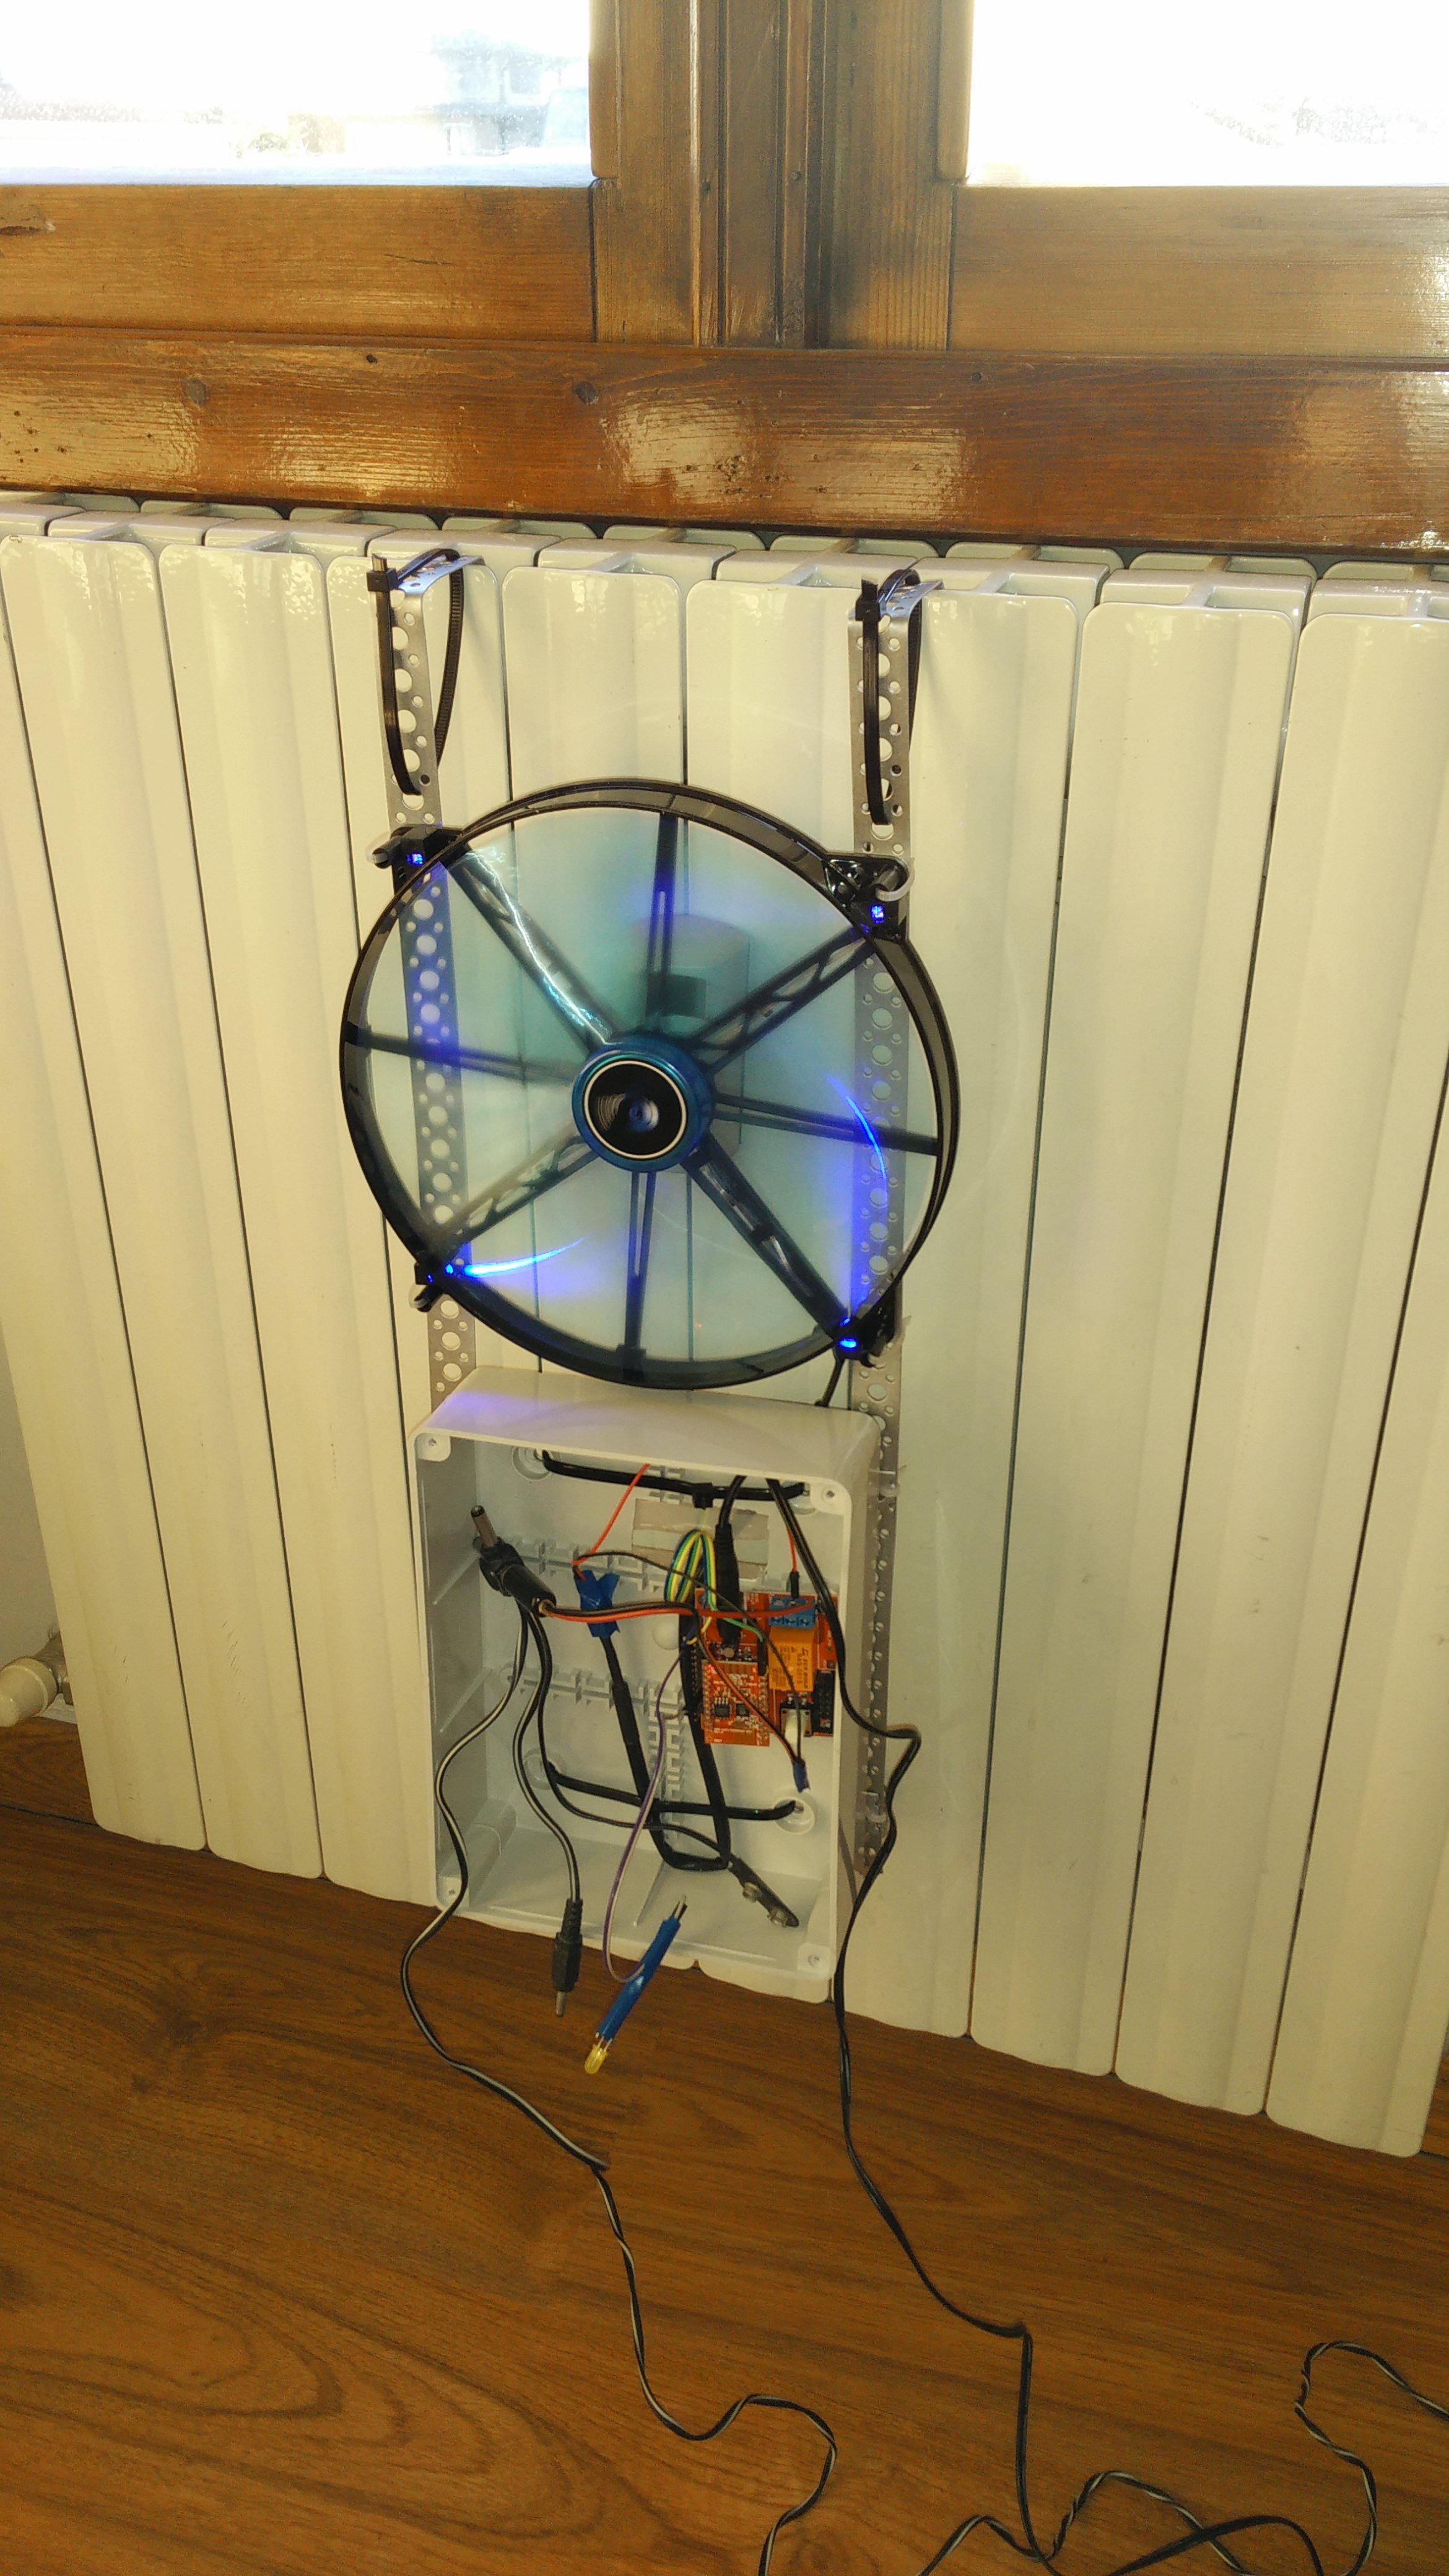
\includegraphics[height=0.5\textheight]{../docs/img/2016-02-04_16.03.52}
	\caption{versione originale}
	\label{fig:originale}
\end{figure}

\begin{itemize}
	\item ``Efficientatore'' (versione full)
	\item ``fregatore'' (versione mini) 
	\item ma anche misuratore consumo caloriferi (temperatura al calorifero è un proxy del conteggio)
	\item consumo ventilatore circa 50W al max
	\item iniziato tanti anni fa... (figura \ref{fig:originale})
	\item esp8266 con relè (figura \ref{fig:cuore})
	\item DHT
	\item esphome con ``thermostat'' component (COOL mode)
	\item versione ``presa comandata'' (figura \ref{fig:presa}) montato al calorifero (figura \ref{fig:montaggiofinale})
\end{itemize}

\begin{figure}
	\centering
	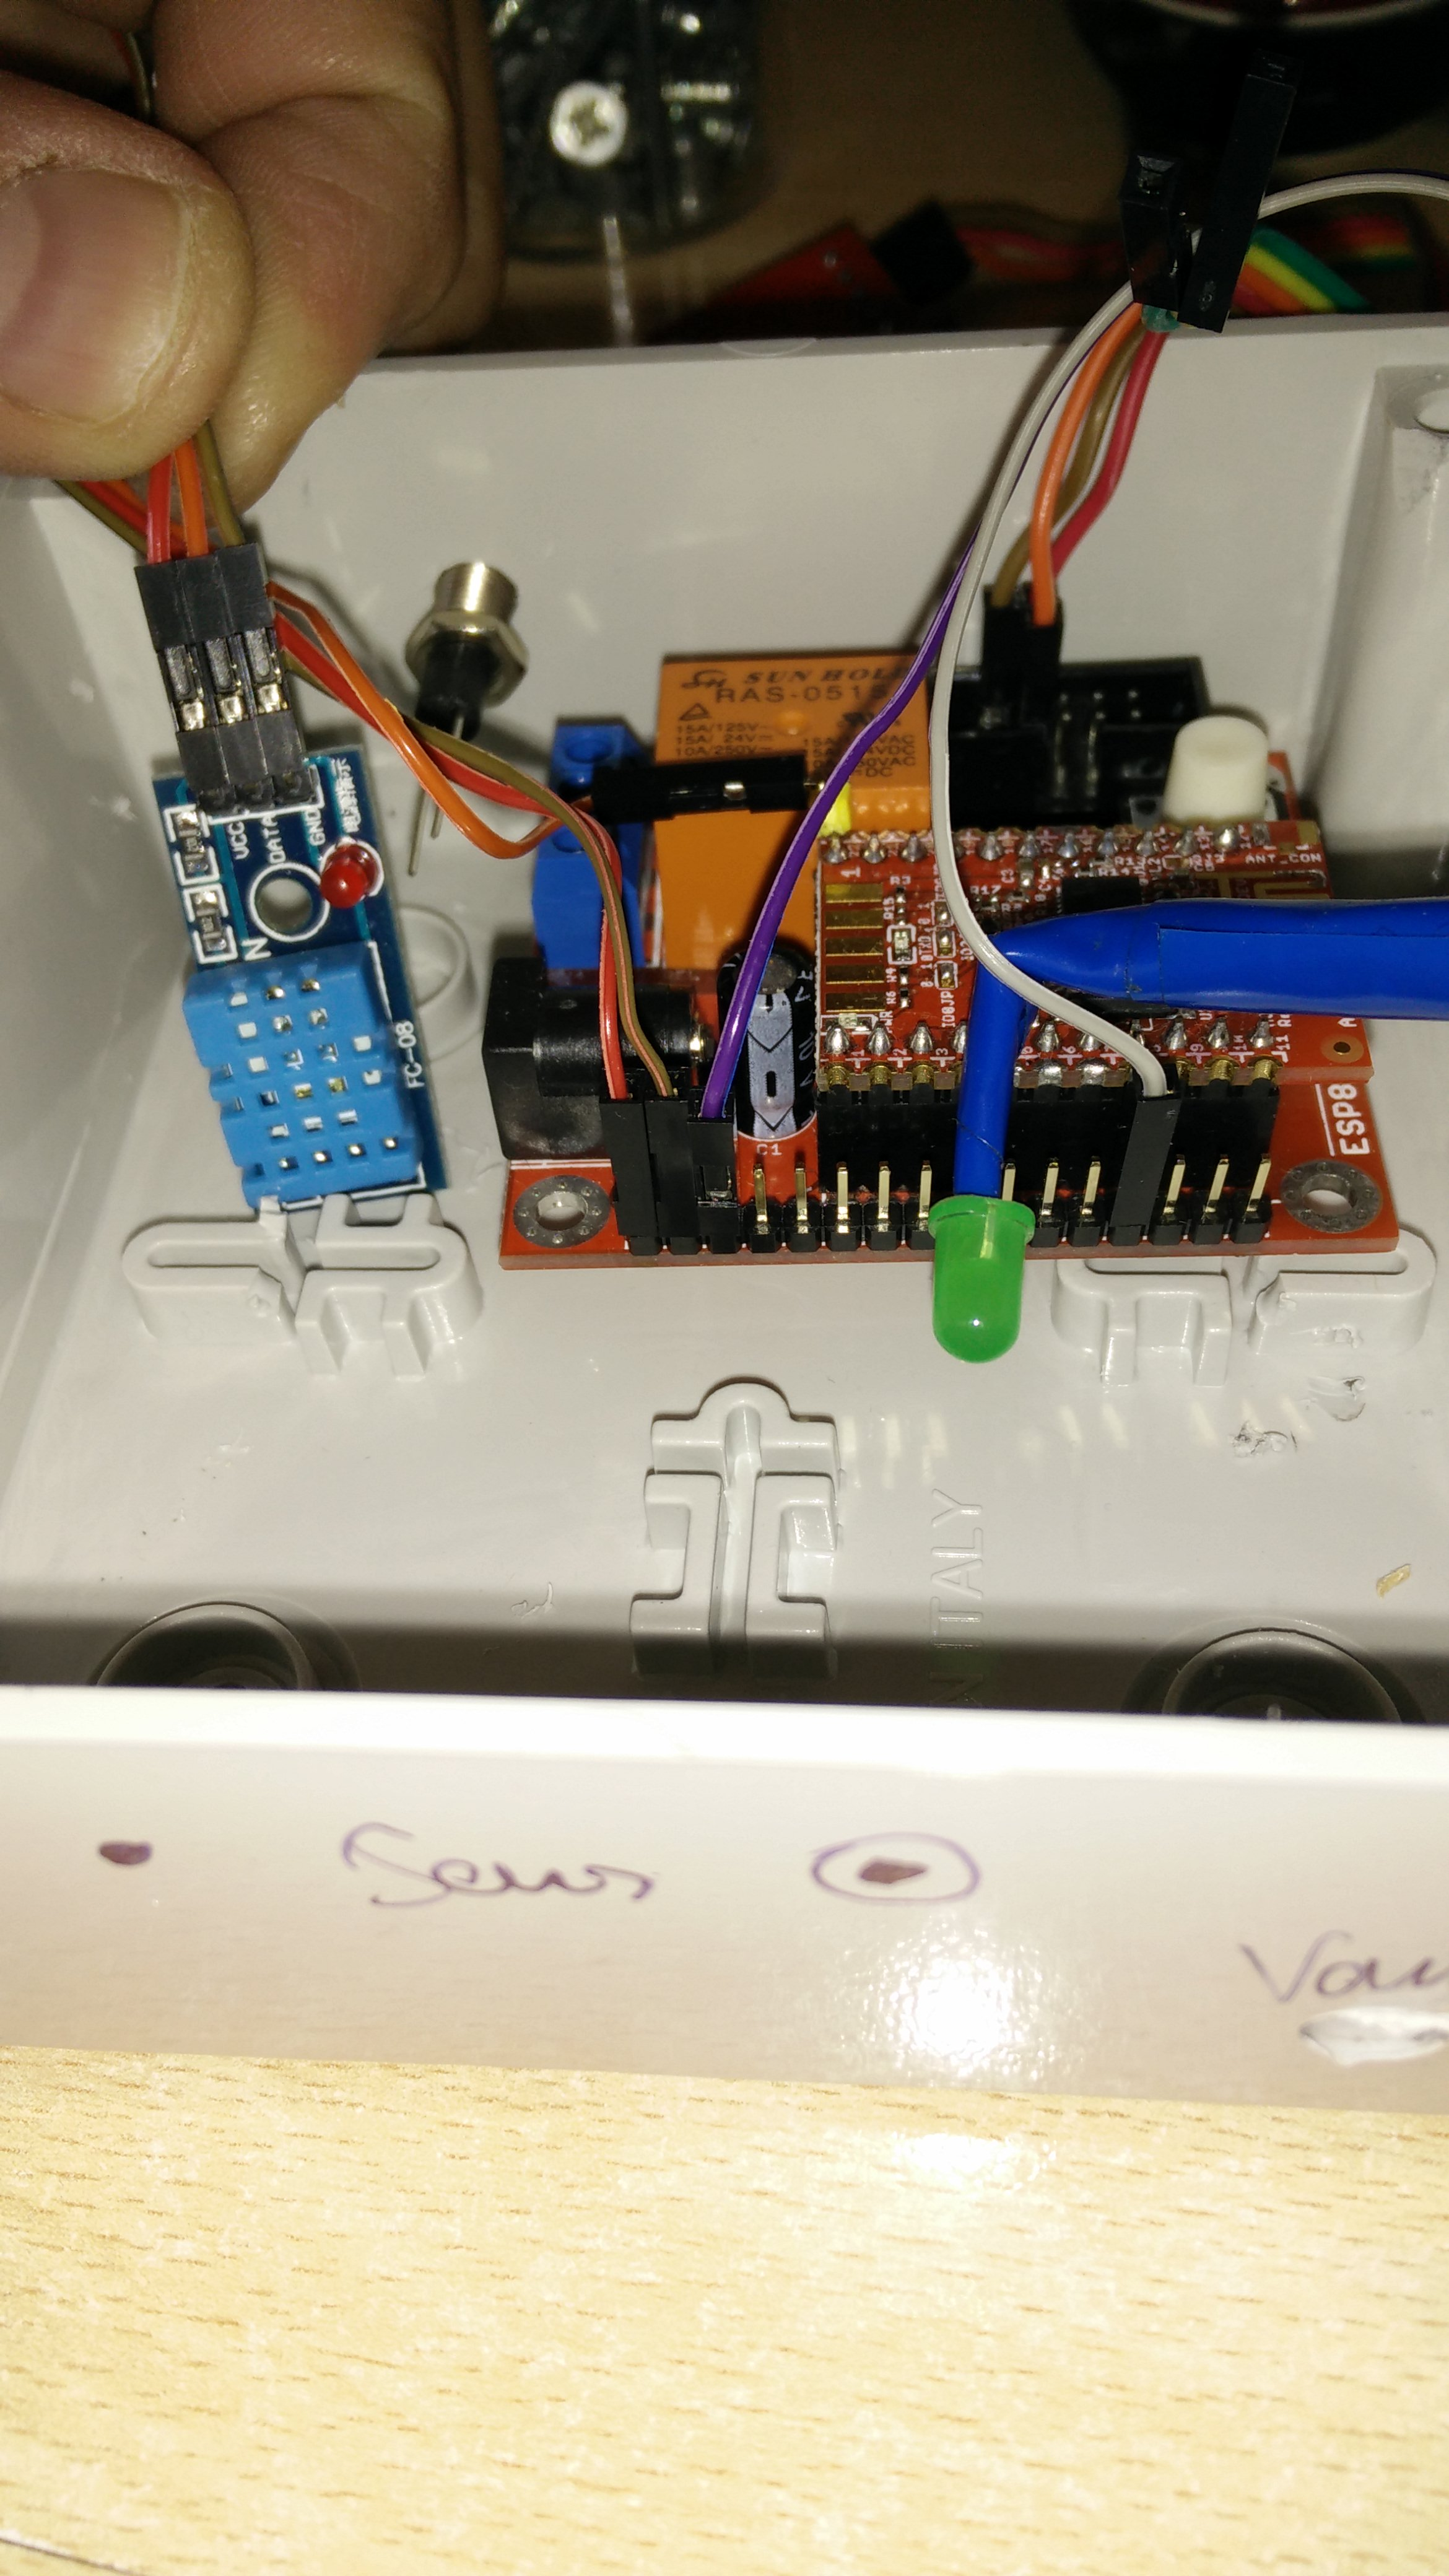
\includegraphics[height=0.4\textheight]{../docs/img/2016-03-21_16.06.25}
	\caption{cuore (esp8266 Olimex)}
	\label{fig:cuore}
\end{figure}

\begin{figure}
	\centering
	\includegraphics[width=0.3\linewidth]{../LabTermuinator/img/2023-01-15_18.09.04.jpg}
	\caption{versione ``presa comandata''}
	\label{fig:presa}
\end{figure}

Sorgente esphome:
\lstinputlisting{~/IN-CORSO/TermuinatorOlimex/EsphomeVersion/termuinator.yaml}

\begin{figure}
	\centering
	\includegraphics[angle=-90,width=0.4\linewidth]{../LabTermuinator/img/2023-01-16_16.42.59}
	\caption{montaggio finale termuinator}
	\label{fig:montaggiofinale}
\end{figure}


%%%%%%%%%%%%%%%%%%%%%%%%%%%%
\section{Cam di lettura contacalorie}

\begin{itemize}
	\item lettura a vista cmq difficoltosa (figura \ref{fig:letturadifficoltosa})
	\item esp32cam + usbprogrammer
	\item esphome
	\item flash led programmato tarda serata (campionamento dopo le 23)
	\item vibrazione dovuta al fan bloccata con gommapiuma (figura \ref{fig:cam})
	\item motion (on openwrt, tuning diff!!!)
	\item syncthing (sync dei file)
\end{itemize}

\begin{figure}
	\centering
	\includegraphics[angle=180,width=.6\linewidth]{../LabTermuinator/img/2022-11-26_18.45.54}
	\caption{lettura difficoltosa}
	\label{fig:letturadifficoltosa}
\end{figure}

\begin{figure}
	\centering
	\includegraphics[width=\textwidth]{"../LabTermuinator/img/2023-02-15_14.25.25"}
	\caption{Cam versione definitiva}
	\label{fig:cam}
\end{figure}

Sorgente esphome:
\lstinputlisting{~/IN-CORSO/ESP32-CAM/cam.yaml}


Script stats.sh (stats generazione immagini, per aiutare nel tuning motion+flashing):
\begin{lstlisting}
for dir in $(find -name 'term*' | cut -f-4 -d/ | sort | uniq); do
	echo $dir
	ls $dir/term* | cut -f3 -d_ | cut -f1 -d: | sort -n | uniq -c | tr -s " " | awk '{print $2,$1}'
done
\end{lstlisting}


\begin{lstlisting}
./2023/02/14
00 110
01 106
02 111
03 110
04 126
05 123
06 110
07 139
08 145
09 152
10 130
11 168
12 131
13 142
14 190
15 118
16 147
17 133
18 114
19 101
20 108
21 102
22 105
23 108
./2023/02/15
00 118
01 116
02 112
03 109
04 103
05 124
06 118
07 125
08 166
09 143
10 142
11 146
12 120
13 135
14 229
15 125
16 205
17 126
18 115
19 113
20 117
21 115
22 105
23 100
...
./2023/02/23
00 110
01 130
02 125
03 125
04 113
05 122
06 120
07 130
08 136
09 138
10 153
11 144
12 149
13 110
14 361
15 13
16 22
17 53
18 2
23 30
./2023/02/24
00 6
03 8
07 9
08 16
09 47
10 15
11 12
12 38
13 31
14 25
15 11
16 67
17 145
18 64
23 20
...
\end{lstlisting}

%%%%%%%%%%%%%%%%%%%%%%%%%%%%%%%%%%%%%%%%%
\section{Digressione misura consumo traffico dati VeryMobile}
\begin{itemize}
\item VeryMobile NON ha API di consultazione traffico residuo, né un meccanismo via web, solo APP (inserire bestemmie)
\item ergo ci vuole ADB + screenshot (figura \ref{fig:screenshot})
\item OCR (tesseract) per estrarre il dato
\end{itemize}

Script ADB screenshot:
\begin{lstlisting}
#!/bin/bash

cd /Syncthing/atrent-condivisione/LabCellScreens

adb shell input keyevent 26 && adb shell input touchscreen swipe 930 880 930 380 && adb shell input text XXXXX && adb shell input keyevent 66

adb shell monkey -p it.very.mobile -c android.intent.category.LAUNCHER 1 

sleep 30

echo ...capture...
adb exec-out screencap -p > $(date +%Y-%m-%d_%H:%M).png

sleep 10

#adb shell monkey -p fr.neamar.kiss -c android.intent.category.LAUNCHER 1 

# home & kill
echo ...exit...
adb shell input keyevent 4
adb shell am force-stop it.very.mobile
\end{lstlisting}



\begin{figure}
	\centering
	\includegraphics[height=.5\textheight]{~/atrent-condivisione/LabCellScreens/2023-03-15_18:42}
	\caption{screenshot}
	\label{fig:screenshot}
\end{figure}



Estrazione OCR:
\begin{lstlisting}
#!/bin/bash

for img in *.png; do
	OUT=$(basename "$img" .png)
	if ! test -e "$OUT.txt"; then
		tesseract "$img" $(basename "$img" .png)
	fi
done

echo data,gb >ocr.csv
grep -e "[0-9][0-9]\.[0-9]" ./*.txt | cut -f1 -d" " | cut -c3- | sed 's/\.txt:/,/g' | tr "_" " " | sort -n | tee -a ocr.csv

./plot.r

eog *.jpg &
\end{lstlisting}


Script R plot per ottenere figura \ref{fig:plottraffico}:
\begin{lstlisting}
#!/usr/bin/env Rscript
library(anytime)
ocr=read.csv("ocr.csv",sep=",",header=TRUE)
ocr$data <- anytime(ocr$data)
summary(ocr)
jpeg("gb.jpg",width=30,height=15,units="cm",res=300)
plot(ocr$data,ocr$g ,col="red",type="l",ylim=c(0,100))
\end{lstlisting}

\begin{figure}
	\centering
	\includegraphics[width=\textwidth]{~/atrent-condivisione/LabCellScreens/gb.jpg}
	\caption{plot traffico}
	\label{fig:plottraffico}
\end{figure}




%%%%%%%%%%%%%%%%%%%%%%%%%
\section{Temperatura esterna}
\begin{itemize}
\item raspberry pi sul balcone
\item dht
\item log su file
\item presi via scp
\item (difetto) non protetto dal sole diretto
\item è su da anni
\end{itemize}

%%%%%%%%%%%%%%%%%%%%%%%%%%%%
\section{MQTT}
\begin{itemize}
	\item solito atrent.it
	\item script di cattura fatto con mosquitto\_sub +  qualche filtro
	\item save su log file CSV
\end{itemize}


%%%%%%%%%%%%%%%%%%%%%%%%%%%%%%
\section{Riporto letture contacalorie}
\begin{itemize}
\item foglio elettronico
\item interpretazione immagine a vista (OCR tentato senza successo)
\item generazione CSV
\end{itemize}

%%%%%%%%%%%%%%%%%%%%%%%%%%%%%
\section{Plot finale}

Mangia un po' di CSV e plotta (figura \ref{fig:plot}):
\begin{lstlisting}
library(lubridate)
library(anytime)
library(units)

#################################################
t=read.csv("temps.csv",sep=" ",header=TRUE)
t$Data <- as_datetime(t$Data)

c=read.csv("cooling.csv",sep=" ",header=TRUE)
c$Data <- as_datetime(c$Data)

l=read.csv("2plot.csv",sep=",",header=TRUE)
l$timestamp <- as_datetime(l$timestamp)
l$Lcorrente <- l$Lcorrente/20 # scalato
l$Lmezzanotte <- l$Lmezzanotte/15 # scalato
l$dT <- l$dT*2 # scalato

outside = read.csv("outsideTemp.csv")
outside$Data <- ymd_hm(outside$Data)

total <- merge(c,t,by="Data",all.x=TRUE)

summary(total)

jpeg("plot.jpg",width=30,height=15,units="cm",res=300)

plot(total$Data,total$Temp,col="red",type="l",ylim=c(-1,45),xtitle=NULL)

points(l$timestamp,l$Lcorrente,col="blue")
par(las=2)
axis.POSIXct(1, at=l$timestamp, labels=format(l$timestamp, "%d/%m"))

abline(lm(l$Lcorrente ~ l$timestamp),col="yellow")

lines(l$timestamp,l$Diff24,col="magenta")

lines(outside$Data,outside$temp,col="cyan")
grid(nx = NULL, ny = NULL,
lty = 2,      # Grid line type
col = "gray", # Grid line color
lwd = 1)      # Grid line width

lines(total$Data,total$Action)
\end{lstlisting}


\begin{figure}
	\centering
	\includegraphics[width=\textwidth]{../LabTermuinator/plot}
	\caption{risultato finale}
	\label{fig:plot}
\end{figure}



\section{Migliorie possibili}

\begin{itemize}
\item posizionare temperatura esterna a nord

\item mettere altri sensori temp in lab per confronto e check solare

\item BME280 invece di DHT

\item sensore temp calorifero ad appoggio (sonda), es. LM35

\item wireguard e PULL (scp dei log, chirurgico) invece di PUSH (syncthing)

\item nodered per processare direttamente i msg invece di passare per i csv (dallo stream mqtt)

\item lettura RF del contacalorie (provata con tesista qualche anno fa, senza successo, ho la board, ma complicata)

\item calcolare/prevedere direttamente i consumi in funzione della temperatura misurata al calorifero (i.e., clono la funzionalità del contacalorie: integrazione temperatura/dT)

\item lettura consumo fan (magari via sonoff)

\item si può scorporare le varie componenti: avere solo un termometro e solo una fan comandabile, che si parlano in MQTT, logica distribuita o centralizzata (HomeAssistant?)

\end{itemize}

\end{document}
